In this section, we evaluated our proposed method against other methods in the literature. From previous research about fault diagnosis in WSNs, we selected  Deep Belief Network \cite{Prasad2023}, LSTM-AE \cite{Khan2024}, and Support Vector Machine(SVM).

\subsection{Dataset}
For purpose of fault detection, we created an original dataset using data from NASA MERRA-2 reanalysis data (Temperature at 2 Meter) as substitution for measurements taken from a WSN \cite{GMAO2015}. The data is collected from the North Vietnam region from a period of roughly 6 months. Another dataset used for performance evaluation is the Intel Lab Dataset. This dataset comprises readings from a network of 54 sensor nodes, specifically Mica2Dot devices, which were outfitted with environmental sensing capabilities. These nodes systematically captured time-stamped information relating to ambient conditions, including temperature, humidity, light levels, and the sensors' own voltage. The data acquisition process occurred at intervals of roughly 31 seconds for each sensor. The collection period for this particular dataset extended from late February 2004 through early April 2004 \cite{Intel2004}.

\subsection{Metrics}
To evaluate the performance of the proposed HiFiNet and compare it with other methods, several standard classification metrics are employed. These metrics are calculated based on the number of true positives (TP), false positives (FP), true negatives (TN), and false negatives (FN) for each class. In a multi-class classification problem, these are often computed for each class $c_i$ in a set of classes $C = \{c_1, c_2, \dots, c_K\}$.

Given that \(TP_i\) is the number of true positives for class \(c_i\), \(FP_i\) is the number of false positives for class \(c_i\), \(FN_i\) is the number of false negatives for class \(c_i\), \(N\) is the total number of instances, \(N_i\) is the number of true instances belonging to class \(c_i\).

Accuracy measures the overall correctness of the classifier. It is the ratio of the number of correctly classified instances to the total number of instances.
\begin{equation}
  \text{Accuracy} = \frac{\sum_{i=1}^{K} TP_i}{N}
\end{equation}

Next, precision measures the proportion of positively predicted instances for class \(c_i\) that were actually correct. It is calculated as the ratio of true positives for class \(c_i\) to the sum of true positives and false positives for class \(c_i\).
\begin{equation}
  \text{Precision}_i = \frac{TP_i}{TP_i + FP_i}
\end{equation}
The weighted average precision is computed as:
\begin{equation}
  \text{Weighted Precision} = \sum_{i=1}^{K} \left( \frac{N_i}{N} \times \text{Precision}_i \right)
\end{equation}

Finally, the F1-score is the harmonic mean of precision and recall for a class \(c_i\), providing a single score that balances both concerns.
\begin{equation}
  \text{F1-score}_i = 2 \times \frac{\text{Precision}_i \times \text{Recall}_i}{\text{Precision}_i + \text{Recall}_i}
\end{equation}
Similarly, the weighted average F1-score is calculated by:
\begin{equation}
  \text{Weighted F1-score} = \sum_{i=1}^{K} \left( \frac{N_i}{N} \times \text{F1-score}_i \right)
\end{equation}

\subsection{Experiment Parameters}

\subsection{Evaluation Result}
The overall classification accuracy, shown in Figure~\ref{fig:accuracy}, demonstrates a substantial uplift from HiFiNet. HiFiNet maintains a \(2\sim6\%\) accuracy advantage over the second-best model LSTM-AE. SVM and DBN lag behind with sub \(90\%\) and sub \(80\%\) accuracies respectively across datasets. More importantly, the accuracy of HiFiNet does not degrade significantly as fault rate increases when compared to other methods. This indicates that information from neighbors collected in HiFiNet has a major impact in stabilizing the performance when noise becomes more prevalent

\begin{figure}
  \centering
  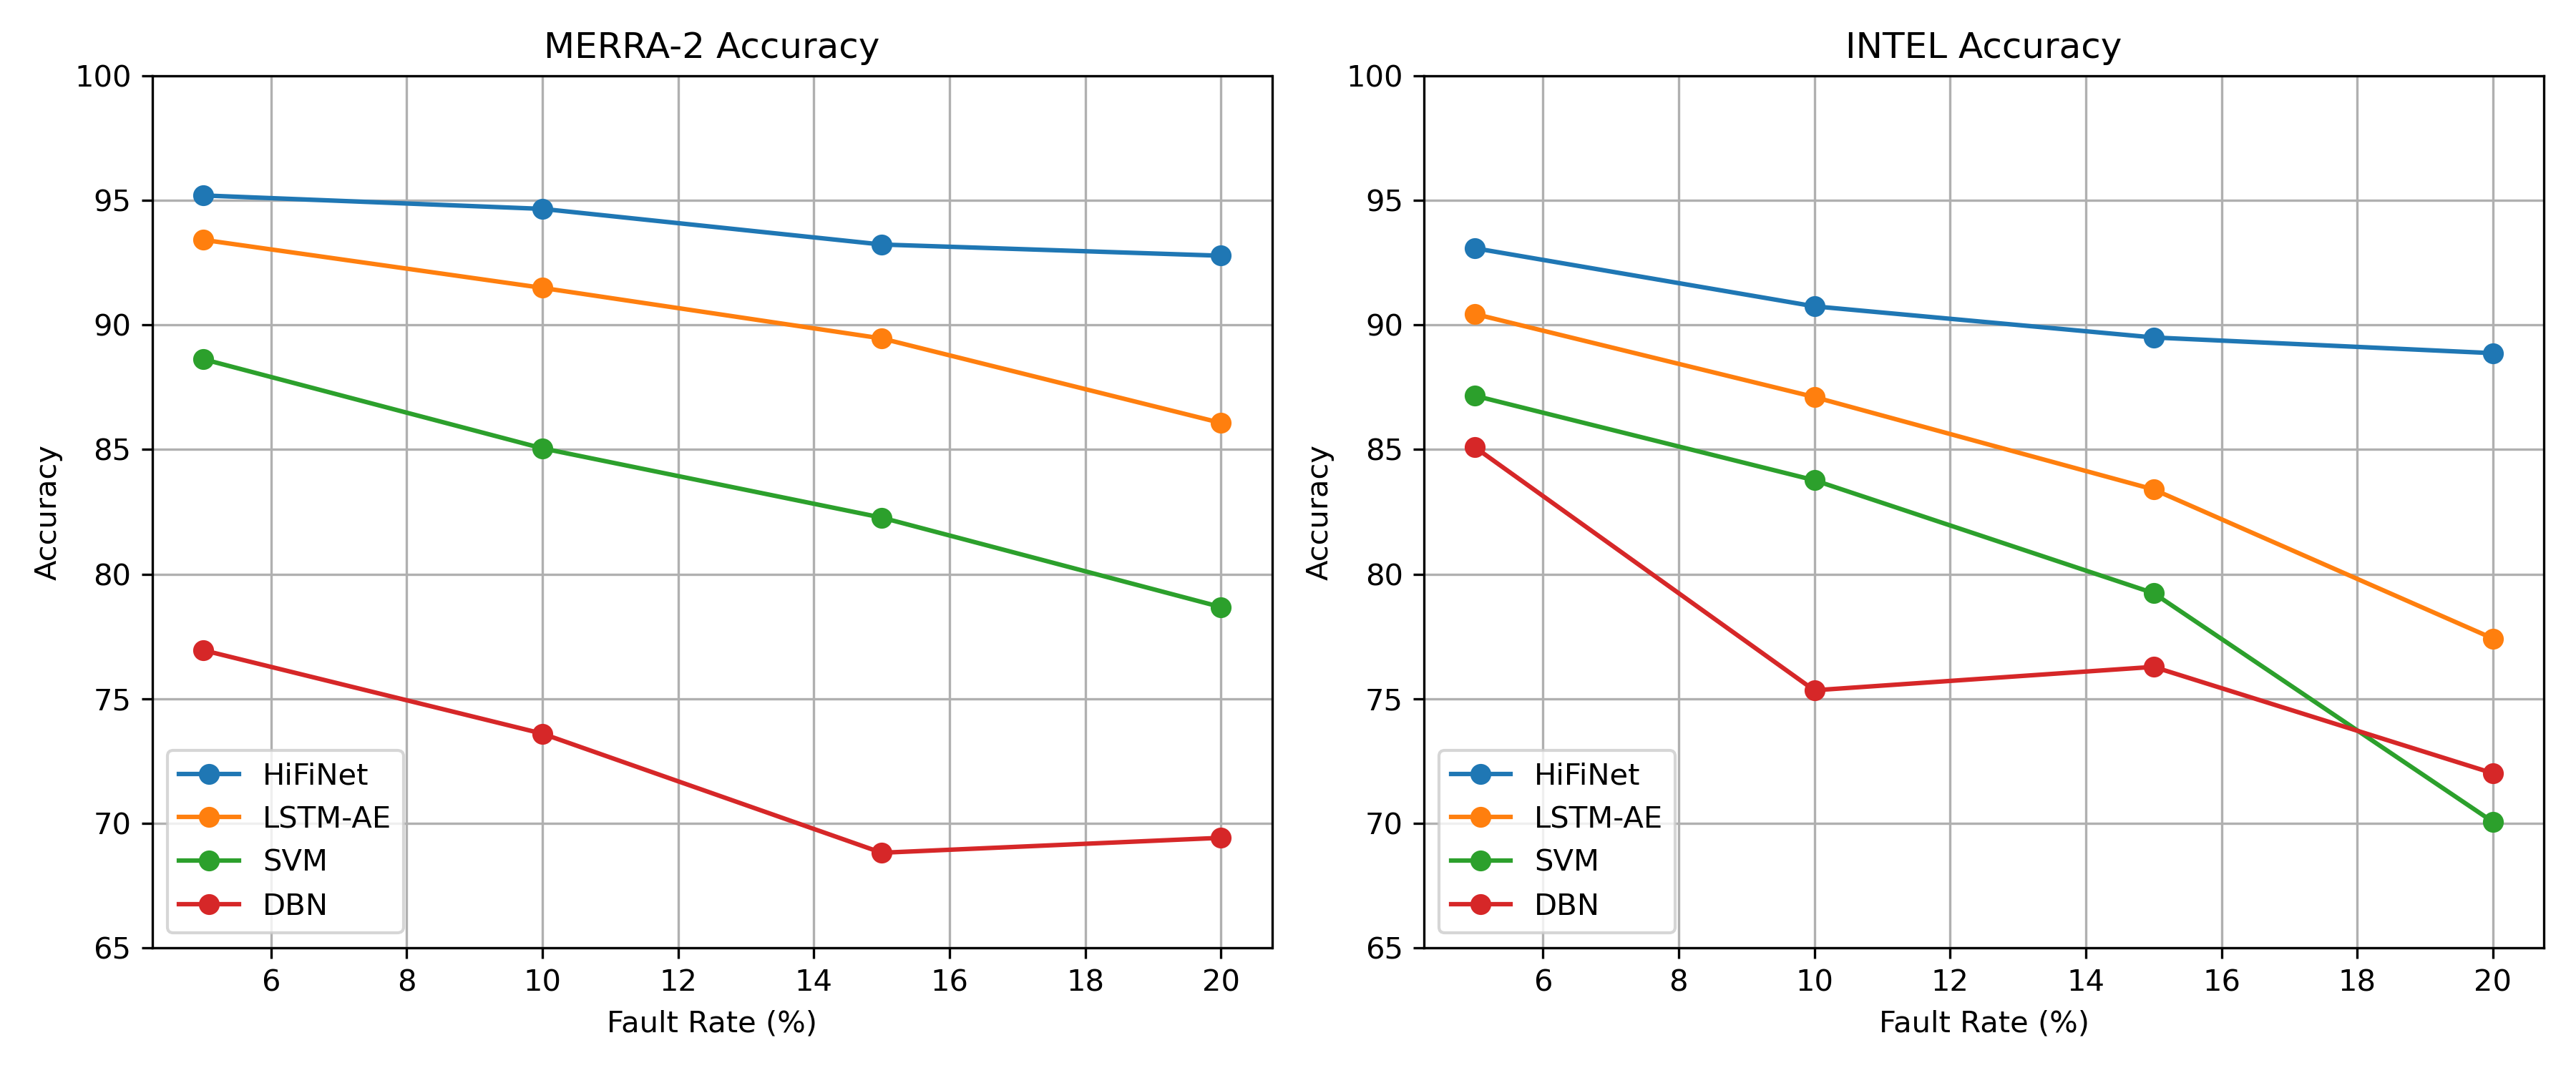
\includegraphics[width=\linewidth]{images/accuracy.png}
  \caption{Accuracy versus Fault Rate comparison between HiFiNet and other methods.}
  \label{fig:accuracy}
\end{figure}

Figure~\ref{fig:f1} plots the F1-Score against the rising fault rates. This further reinforce HiFiNet robustness under noisy condition. HiFiNet achieve upwards of \(94.70\%\) and \(92.32\%\) for MERRA-2 and Intel \(5\%\) fault rate datasets respectively. Compare to LSTM-AE, SVM and DBN, this means a performance delta of \(2\)-\(20\%\) and \(4\)-\(16\%\) on the corresponding datasets, with other fault rate datasets following a similar story. These results suggests that temporal and spatial features utilization has contributes significantly to HiFiNet ability to accurately diagnose each class.

\begin{figure}
  \centering
  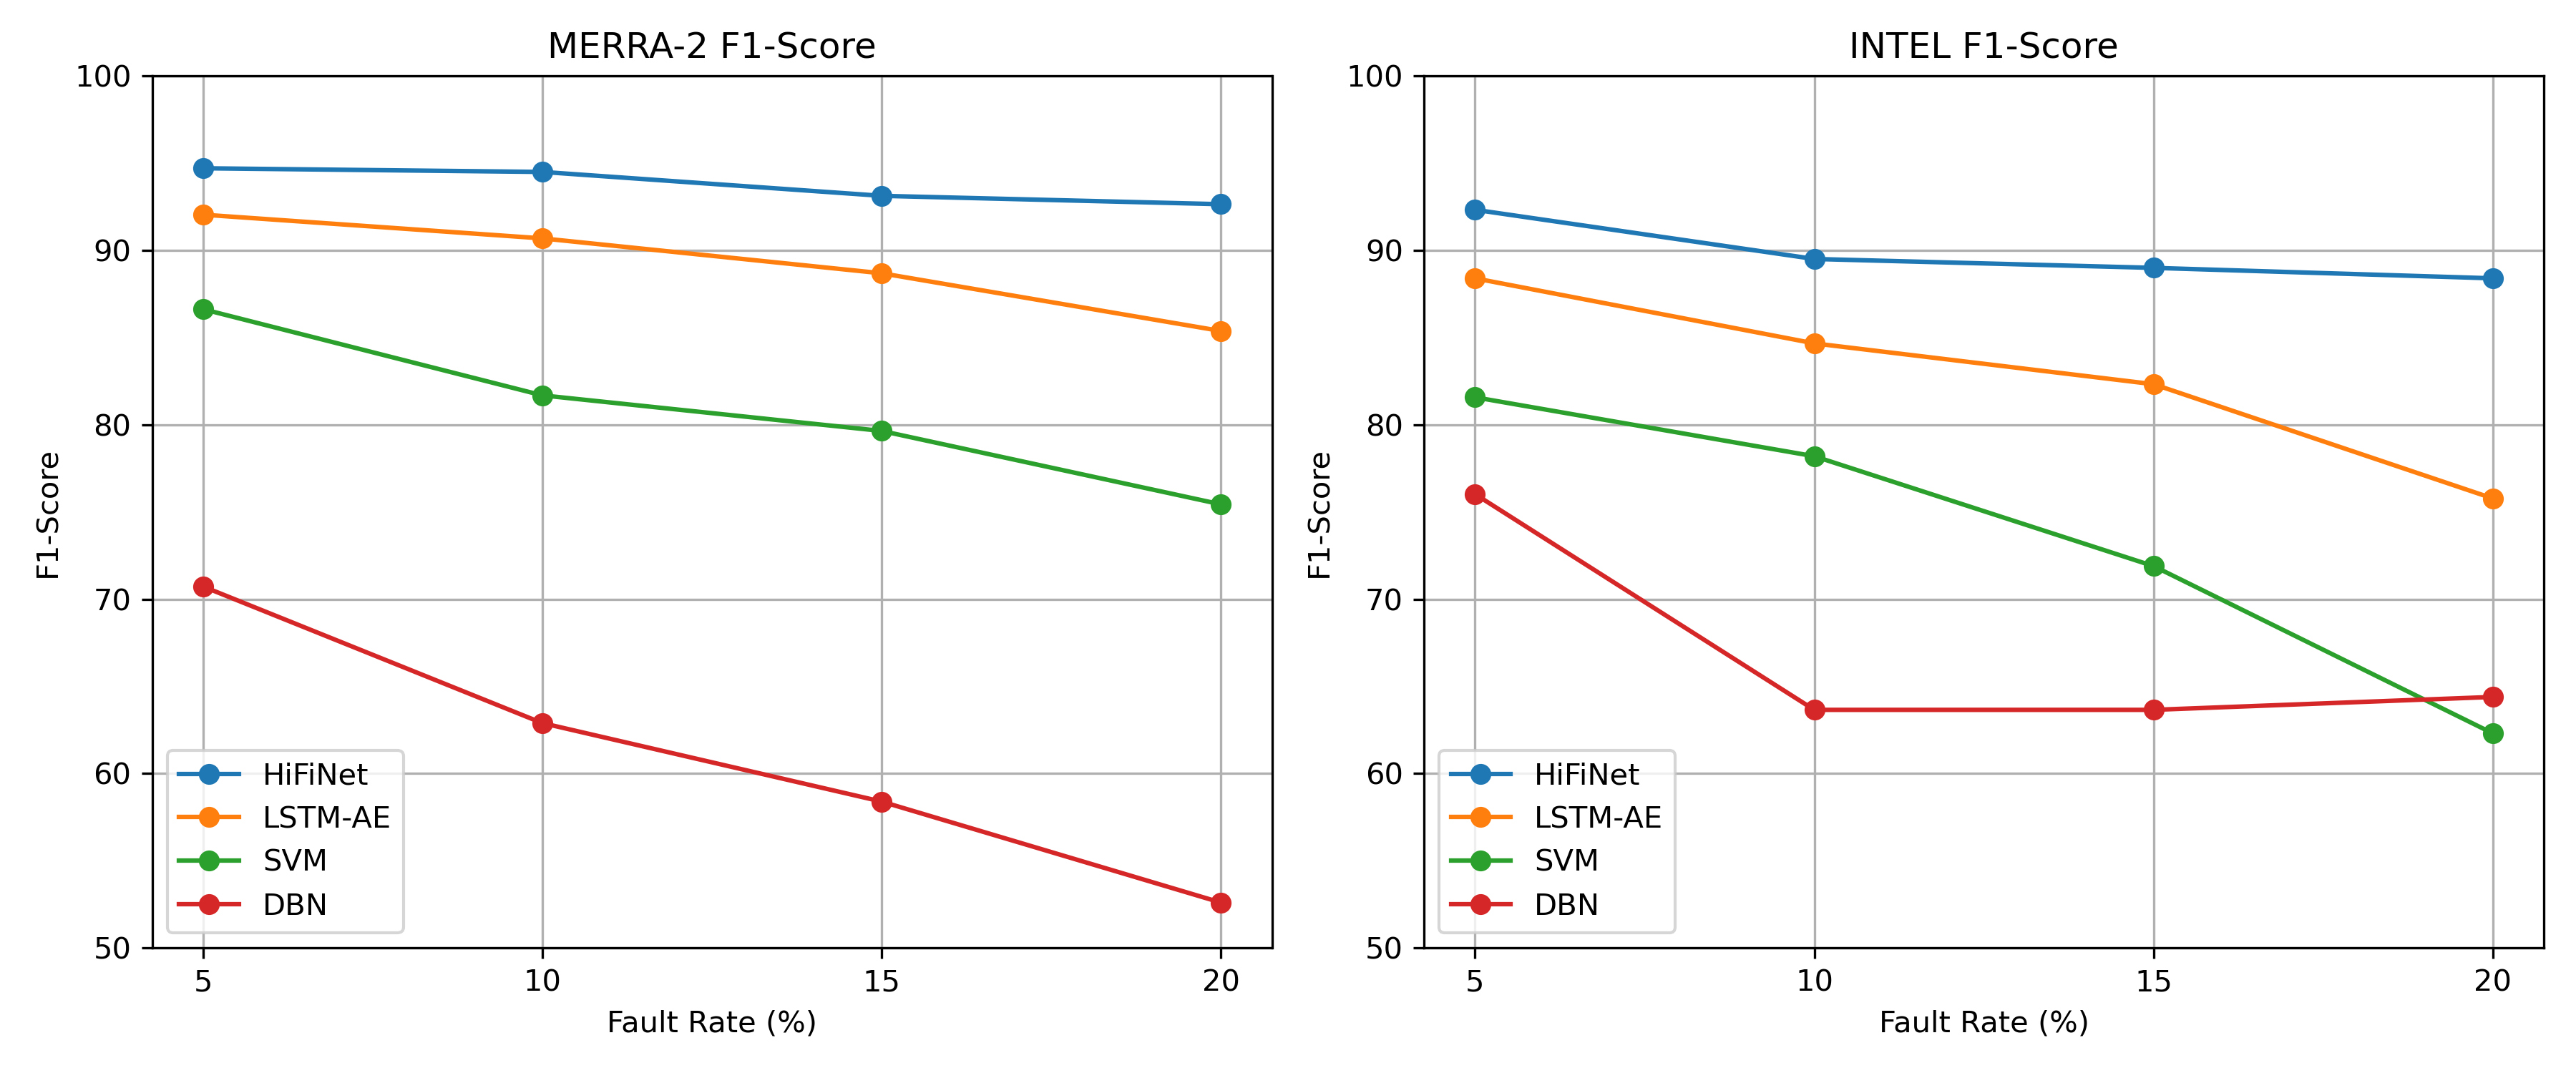
\includegraphics[width=\linewidth]{images/f1.png}
  \caption{F1-Score versus Fault Rate comparison between HiFiNet and other methods.}
  \label{fig:f1}
\end{figure}

To dissect the components of the F1-score, Figure~\ref{fig:pr_scatter} plots Precision versus Recall at the highest stress level (20\% fault rate). An ideal classifier would reside in the top-right corner, signifying perfect precision and recall. For both datasets, HiFiNet is positioned closest to this ideal point. This demonstrates that even in a highly corrupted environment, HiFiNet maintains a superior balance, successfully identifying a high proportion of actual faults (high recall) while simultaneously minimizing the number of false alarms (high precision).

\begin{figure}
  \centering
  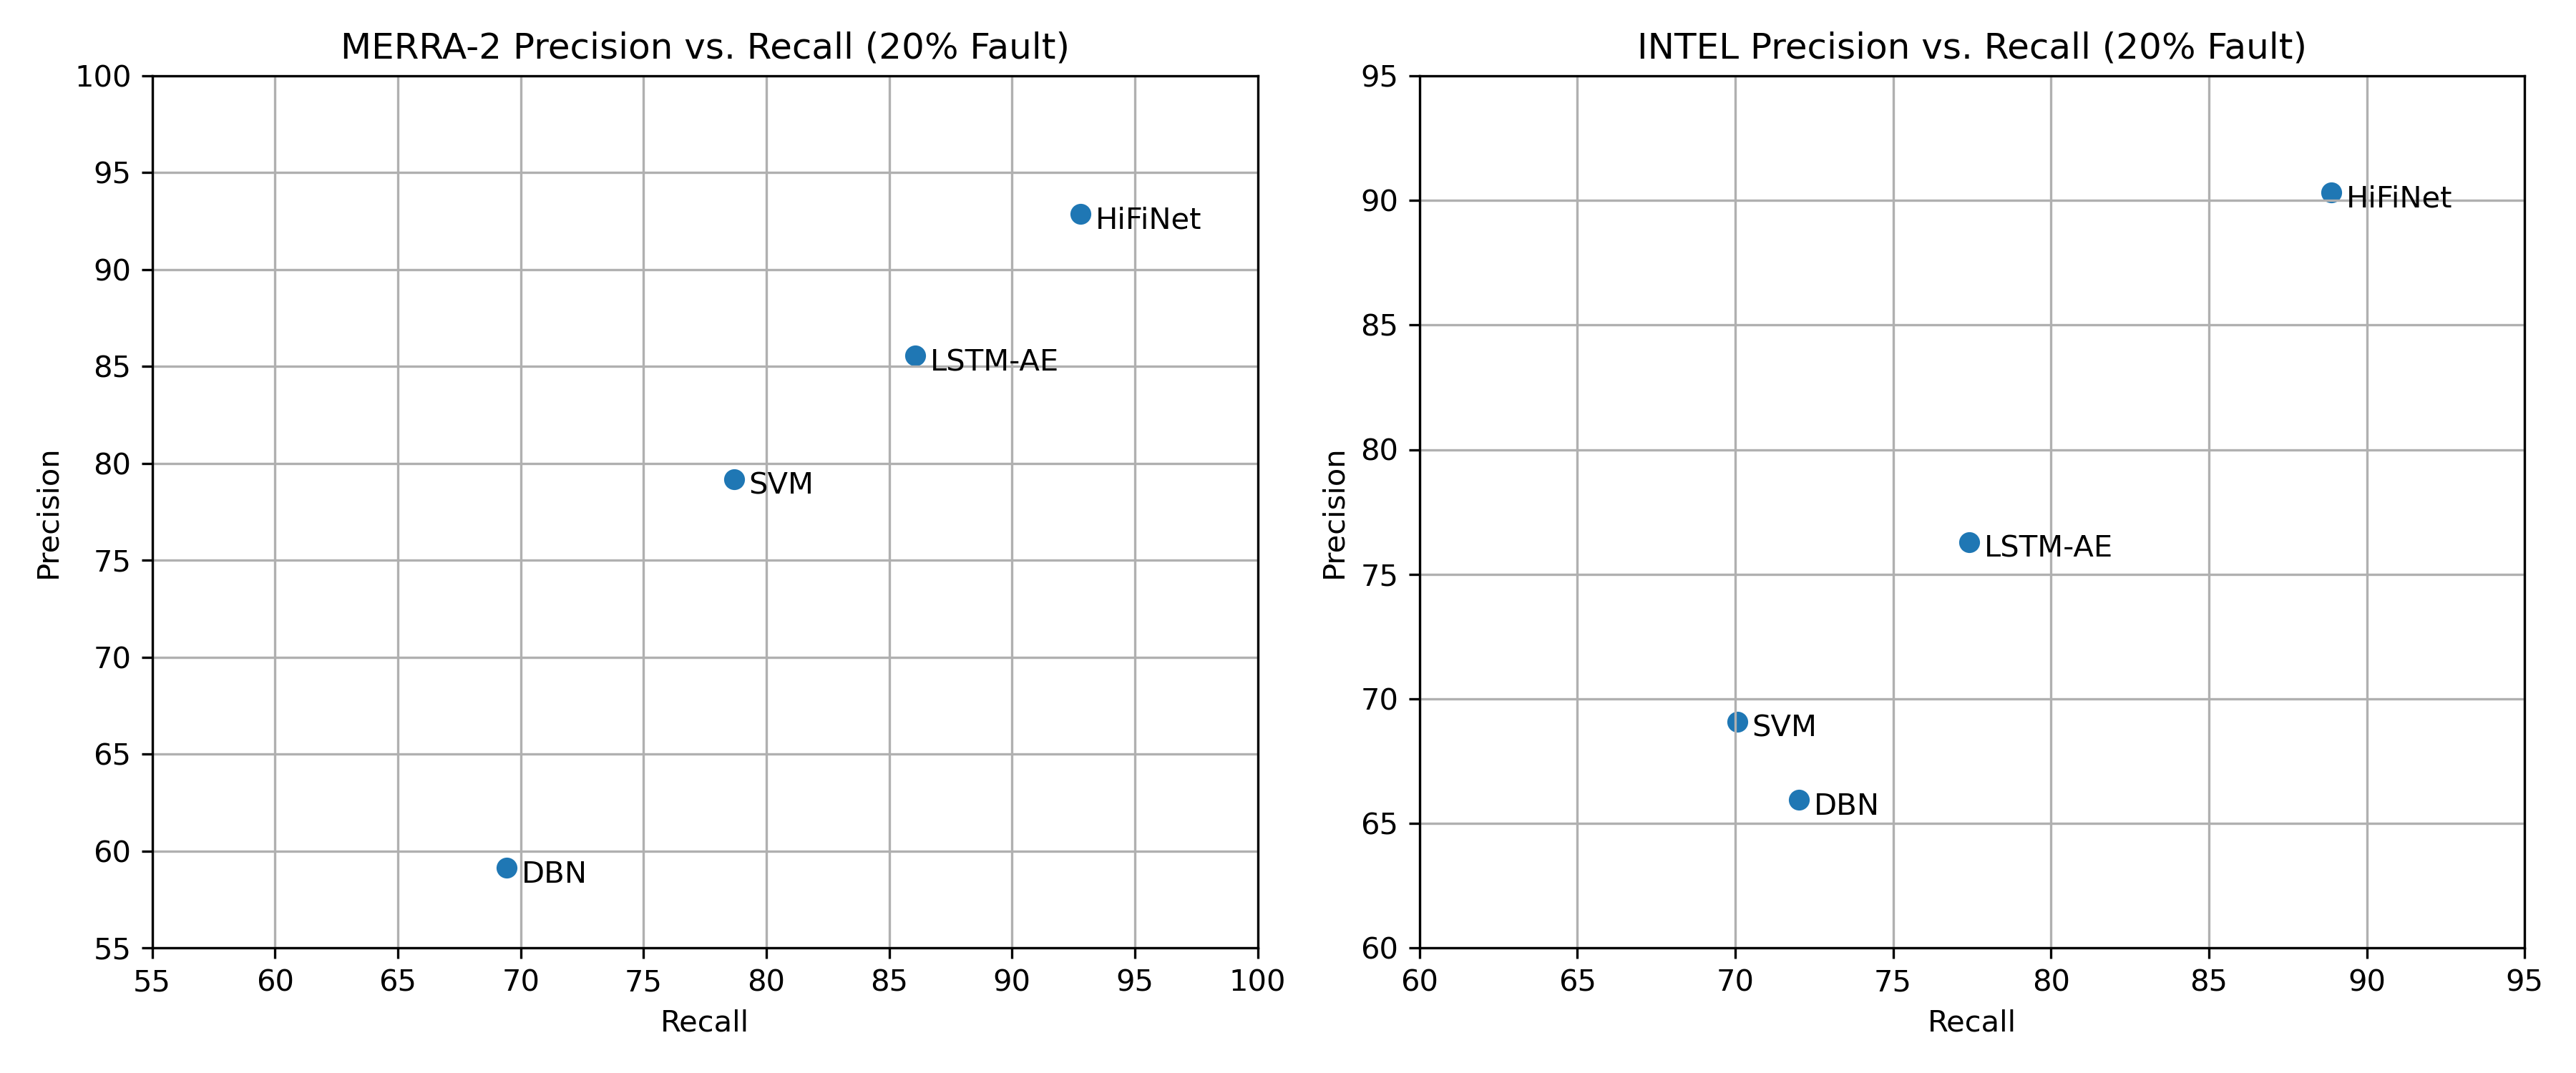
\includegraphics[width=\linewidth]{images/pr_scatter.png}
  \caption{Precision-Recall scatter plot comparison between HiFiNet and other methods. Weight-Average Recall is always equal to Total Accuracy}
  \label{fig:pr_scatter}
\end{figure}

Next, Figure~\ref{fig:f1_drop} provides a direct, quantitative measure of model stability. It visualizes the absolute drop in F1-Score as the fault rate increases from 5\% to 20\%. A smaller bar indicates greater robustness against worsening data quality. HiFiNet clearly stands out with the smallest performance drop on both datasets (2.06 points for MERRA-2 and 3.93 for INTEL). In contrast, models like SVM and LSTM-AE experience much larger drops, exceeding 11 and 12 points, respectively. This bar chart offers a stark visual confirmation of HiFiNet's superior stability and reliability under varying conditions.

\begin{figure}
  \centering
  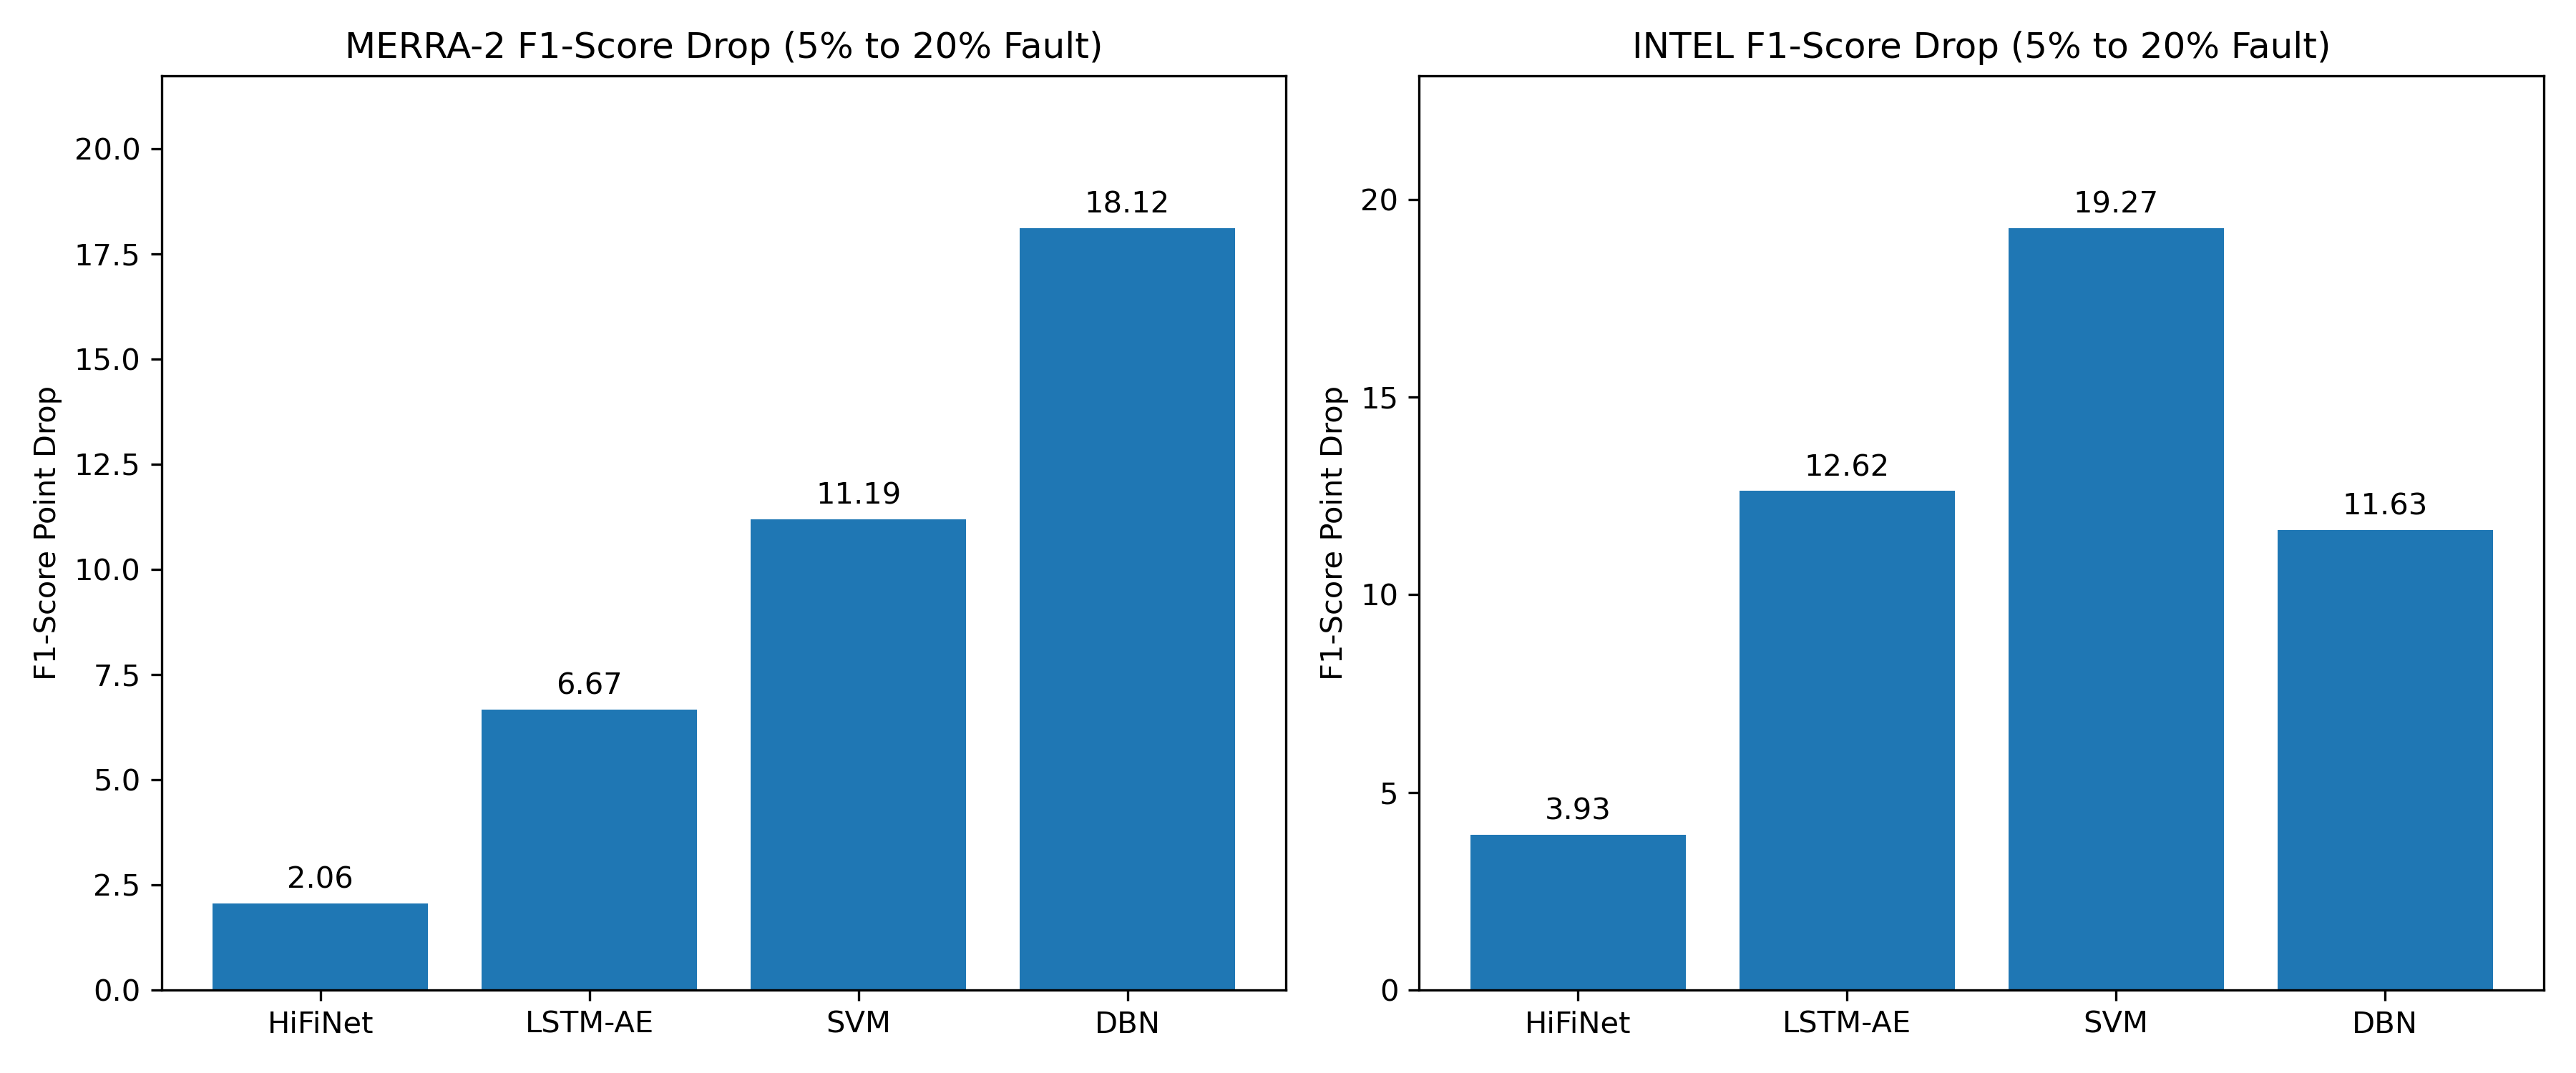
\includegraphics[width=\linewidth]{images/f1_drop.png}
  \caption{F1-Score drop comparison between HiFiNet and other methods.}
  \label{fig:f1_drop}
\end{figure}

While the previous figures provide a visual analysis of key performance trends, tHe complete numerical results for all metrics are consolidated in Table~\ref{tab:metrics} for reference.

\begin{table}
  \centering
  \resizebox{\linewidth}{!}{%
    \begin{tabular}{@{}llrrrrrrrr@{}}
      \toprule
      & & \multicolumn{4}{c}{MERRA-2} & \multicolumn{4}{c}{INTEL} \\
      \cmidrule(lr){3-6} \cmidrule(lr){7-10}
      Metric & Model & 5\% & 10\% & 15\% & 20\% & 5\% & 10\% & 15\% & 20\% \\
      \midrule
      \multirow{4}{*}{Accuracy}
      & HiFiNet   & \textbf{95.20} & \textbf{94.66} & \textbf{93.23} & \textbf{92.78} & \textbf{93.08} & \textbf{90.75} & \textbf{89.50} & \textbf{88.87} \\
      & LSTM-AE   & 93.42 & 91.49 & 89.46 & 86.07 & 90.44 & 87.11 & 83.40 & 77.42 \\
      & SVM       & 88.63 & 85.05 & 82.27 & 78.68 & 87.16 & 83.77 & 79.24 & 70.06 \\
      & DBN       & 76.95 & 73.60 & 68.82 & 69.42 & 85.09 & 75.34 & 76.28 & 72.01 \\
      \midrule
      \multirow{4}{*}{F1-Score}
      & HiFiNet   & \textbf{94.70} & \textbf{94.49} & \textbf{93.12} & \textbf{92.64} & \textbf{92.32} & \textbf{89.50} & \textbf{88.99} & \textbf{88.39} \\
      & LSTM-AE   & 92.04 & 90.68 & 88.68 & 85.37 & 88.39 & 84.66 & 82.32 & 75.77 \\
      & SVM       & 86.62 & 81.68 & 79.64 & 75.43 & 81.57 & 78.19 & 71.89 & 62.30 \\
      & DBN       & 70.72 & 62.89 & 58.39 & 52.60 & 76.02 & 63.65 & 63.65 & 64.39 \\
      \midrule
      \multirow{4}{*}{Precision}
      & HiFiNet   & \textbf{95.21} & \textbf{94.52} & \textbf{93.55} & \textbf{92.89} & \textbf{92.55} & \textbf{91.76} & \textbf{90.16} & \textbf{90.32} \\
      & LSTM-AE   & 92.10 & 90.90 & 89.35 & 85.55 & 89.53 & 86.63 & 82.71 & 76.28 \\
      & SVM       & 86.95 & 82.78 & 81.62 & 79.20 & 76.89 & 73.96 & 67.30 & 69.08 \\
      & DBN       & 70.47 & 60.98 & 53.12 & 59.14 & 72.43 & 66.77 & 57.48 & 65.95 \\
      \bottomrule
    \end{tabular}
  }
  \caption{Comprehensive performance metrics of each method on all datasets.}
  \label{tab:metrics}
\end{table}

\subsection{Ablation Study: Accuracy Tradeoff versus Energy Efficiency of HiFiNet}
To understand the specific contribution of the spatial aggregation component (the Network Classifier) and its associated energy cost, we conducted an ablation study. This analysis investigates the crucial trade-off between the accuracy gained by incorporating neighborhood data and the energy consumed in the process, a primary concern in resource-constrained WSNs. The study's goal is to provide insight into how HiFiNet can be configured for different operational requirements, balancing diagnostic performance with network lifetime.

To quantify the energy cost, we adopt a widely used energy model for WSNs. The model accounts for the energy dissipated during signal transmission, reception, and processing. The combined energy for receiving, aggregating and transmitting data from node \(i\) to node \(j\) is defined by:
\begin{equation}
  E_{t_{ij}} = l (\epsilon_{elec} + \epsilon_{da} + \epsilon_{fs} \cdot d^2_{ij}),
\end{equation}
where \(d_{ij}\) is the distance between nodes \(i\) and \(j\), \(l\) is the number of bits, and \(\epsilon_{elec}\), \(\epsilon_{fs}\), and \(\epsilon_{da}\) represent the energy per bit dissipated in the electronic circuitry of the transmitter or the receiver, the energy cost of transmitting one bit of data over a unit distance squared at short distance, and the energy to aggregate one bit of data.

In our model, we use standard parameter values where \(\epsilon_{elec} = 50\) \si{nJ/bit}, \(\epsilon_{fs} = 10\) \si{pJ/bit/m^2}, \(\epsilon_{mp} = 0.0013\) \si{pJ/bit/m^4}, and the data aggregation energy cost \(\epsilon_{da} = 5 \) \si{nJ/bit}. We define Energy Efficiency (EE) as the inverse of the total energy spent:
\begin{equation}
  EE = 1 / E_{total}.
\end{equation}

The ablation study compares the full HiFiNet architecture against its baseline component: the Edge Classifier operating in isolation (i.e., without the Network Classifier's spatial aggregation). The Accuracy Delta (\%) measures the performance improvement provided by the full HiFiNet over this baseline. We introduce a tunable parameter, Time Delay \(t\), which represents the frequency of execution for the Network Classifier. A time delay of \(t=0\) means the spatial aggregation is performed for every time window processed by the Edge Classifier. A delay of $t=k$ means the aggregation is performed only once every \(k+1\) time windows, using the last known aggregation result for the intermediate steps. The network is assumed to adopt the Constrained Application Protocol (CoAP) with each transmission overhead of 32 bytes. This allows us to control the communication and computation overhead.

The results of this trade-off are presented in Figure~\ref{fig:accuracy_tradeoff}. At a time delay of \(t=0\), the system performs continuous spatial aggregation. This yields the maximum diagnostic benefit, with HiFiNet achieving an Accuracy Delta of over \(3.1\%\) compared to the edge-only model. This configuration, however, is the most energy-intensive, resulting in the lowest Energy Efficiency (approx. 40 units).

\begin{figure}
  \centering
  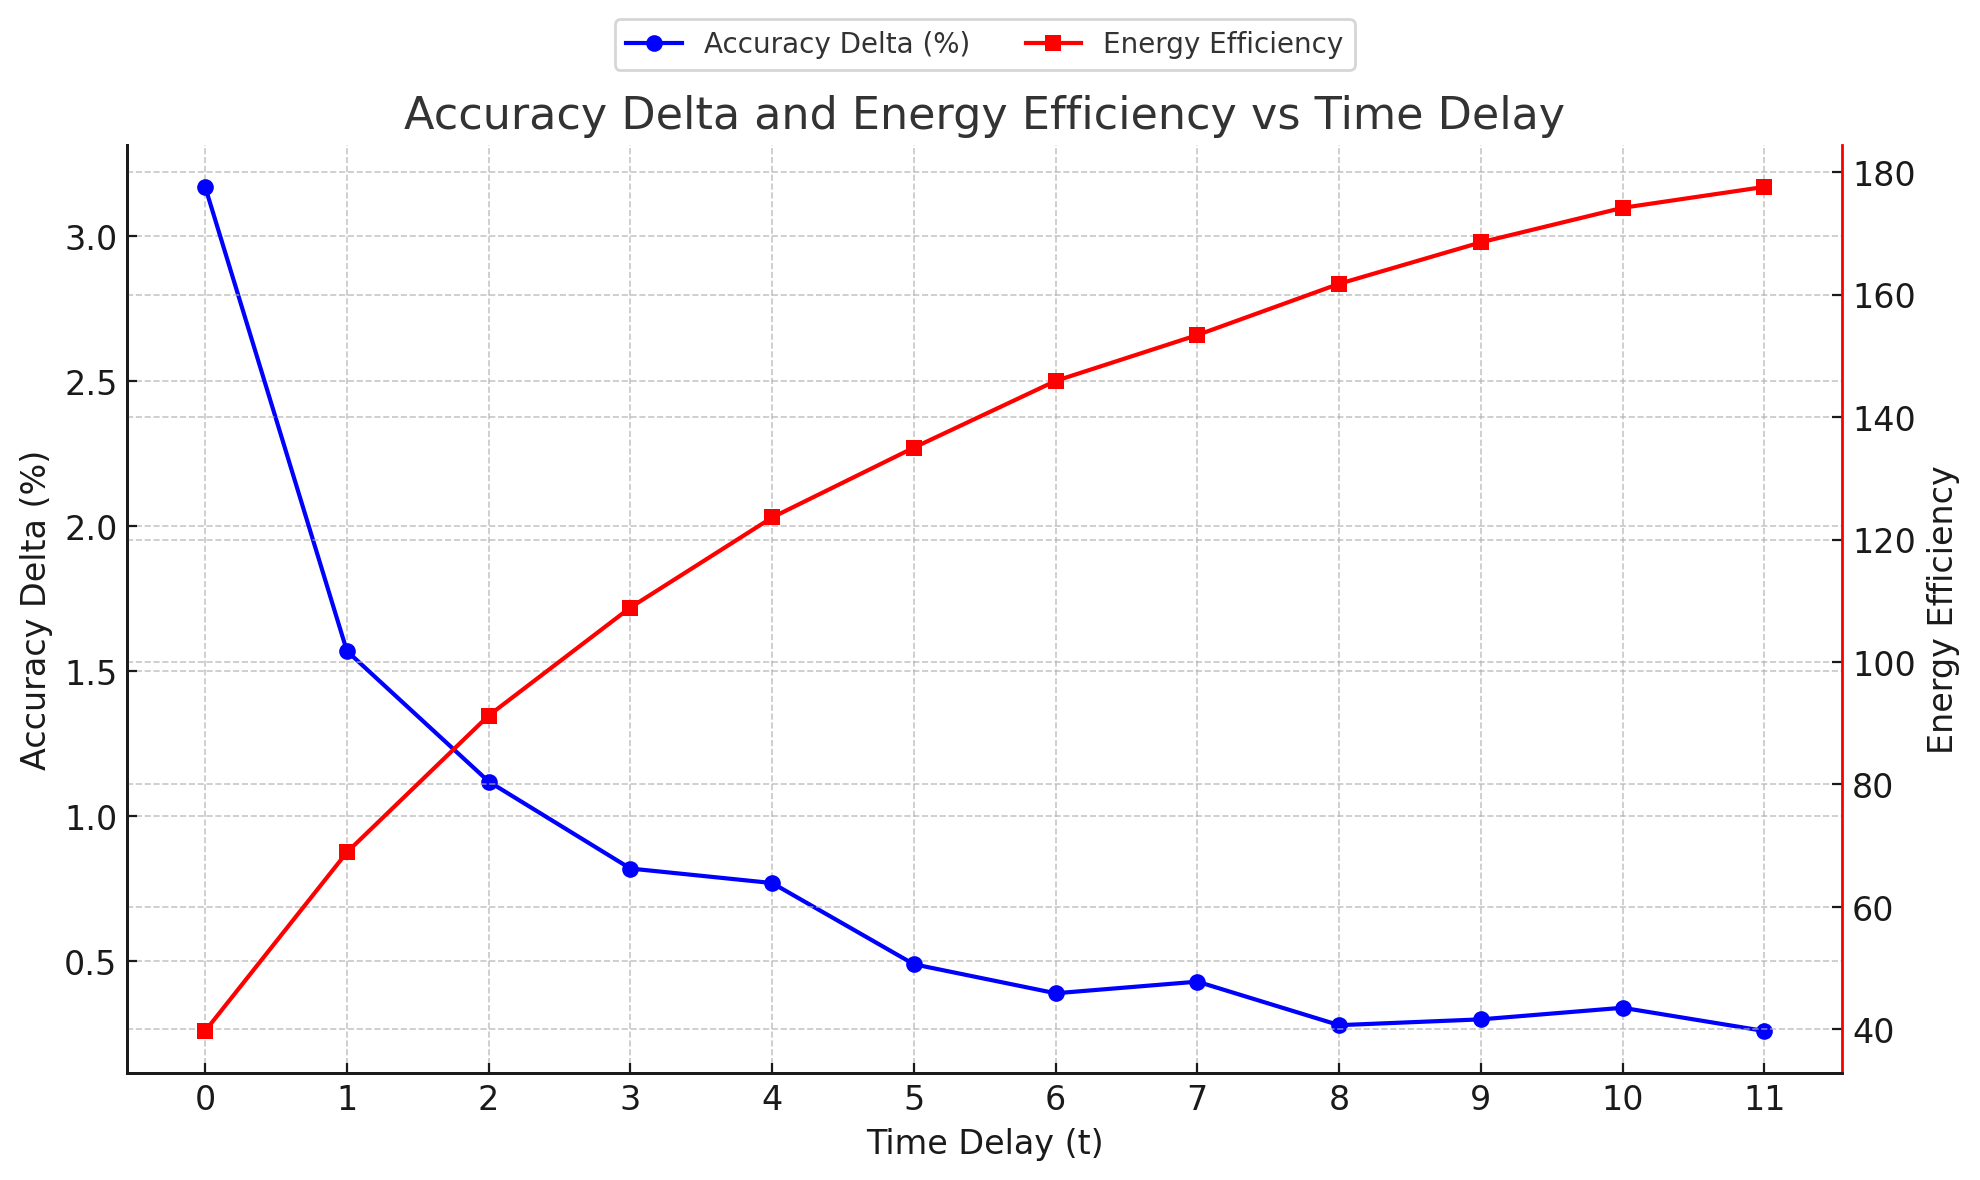
\includegraphics[width=\textwidth]{images/accuracy_tradeoff.png}
  \caption{Accuracy Delta and Energy Efficiency versus Time Delay.  Accuracy Delta represents the performance gain from using the Network Classifier compared to the Edge Classifier alone. Energy Efficiency is inversely proportional to the energy consumed by the communication process.}
  \label{fig:accuracy_tradeoff}
\end{figure}

Conversely, as the Time Delay \(t\) increases, the Network Classifier runs less frequently, drastically reducing the cumulative energy cost. This is reflected in the sharp, monotonic rise of the Energy Efficiency curve, which increases by more than rapidly goes from 0 to 11. This energy saving comes at the cost of accuracy. Since the spatial context is updated less often, its corrective influence diminishes, causing the Accuracy Delta to fall,  and it becomes marginal for $t > 8$.

This analysis reveals that the system's configuration can be optimized based on deployment needs. For critical applications where maximum accuracy is paramount, a low time delay ($t=0$ or $t=1$) is ideal. However, for long-term monitoring where network longevity is the primary concern, a higher time delay (\(t\ge4\)) can provide substantial energy savings with a modest drop in performance. The region between \(t=1\) and \(t=3\) represents a compelling trade-off where a significant portion of the accuracy gain (1.1\%-1.6\%) is retained while achieving a 2-3 times improvement in energy efficiency over the most aggressive configuration. This demonstrates the flexibility of the HiFiNet architecture, allowing operators to tune the model to strike the right balance between diagnostic accuracy and operational lifetime.
